\documentclass[12pt,letterpaper]{article}
\usepackage{./preamble}

%%%%%%%%%%%%%%%%%%%%%%%%%%%%%%%%%%%%%%%%%%
%%%% Edit These for yourself
%%%%%%%%%%%%%%%%%%%%%%%%%%%%%%%%%%%%%%%%%%
\newcommand\course{Computational Statistics}
\newcommand\hwnumber{1}
\newcommand\userID{Davi Sales Barreira}
\DeclareRobustCommand{\rchi}{{\mathpalette\irchi\relax}}
\newcommand{\irchi}[2]{\raisebox{\depth}{$#1\chi$}}

\begin{document}
% \textbf{\Large Worksheet completed with Octave.}

\section*{Exercise 1 (Inversion and Rejection)}
\begin{enumerate}[leftmargin=!,labelindent=5pt]
    \item Let $ F_X(x) = \mathbb{P}(X \leq x) $ and $U \sim Unif[0,1]$:
        % \begin{flalign}
            $$ F_X(x) = 1 - e^{-\lambda(X-a)}\mathbb{I}_{\{X \geq a\}}=U $$
            $$ -\ln(1-U) = \lambda(x-a) $$
            $$ F_X^{-1}(U) = a - \frac{\ln(1-U)}{\lambda} $$
    To simulate X from U, just simulate value from U and substitute in the
    formula above.
        % \end{flalign}
        
    \item Let $X = Y \mid a \leq Y \leq b$.
    First, let's show that $X = F_Y^{-1}(F_Y(a)(1-U)+F_Y(b)U)$:

    % $$p(X=x \mid a \leq X \leq b) = \frac{p(X=x, a \leq X \leq b)}{p()}$$
    $$\mathbb{P}(X \leq x) = \mathbb{P}(F_Y^{-1}(F_Y(a)(1-U)+F_Y(b)U)\leq x)
    = \mathbb{P}(F_Y^{-1}(F_Y(a)+U[F_Y(b)-F_X(a)])\leq x)$$
    % If $x \notin [a,b]$ then $\mathbb{P}(X \leq x) = 0$.
    $$ = \mathbb{P}(F_Y(a)+U[F_Y(b)-F_X(a)]\leq F_Y(x)) = 
    \mathbb{P}\left(U \leq \frac{F_Y(x) - F_Y(a)}{F_Y(b)-F_Y(a)}\right)
    =\frac{F_Y(x) - F_Y(a)}{F_Y(b)-F_Y(a)}$$

    Note that since $x \in [a,b]$: 
    $$\mathbb{P}(Y \leq x \mid a \leq Y \leq b)
    = \frac{\mathbb{P}(Y \leq x, a \leq Y \leq b)}
    {\mathbb{P}(a \leq Y \leq b)}
    =\frac{\mathbb{P}(a \leq Y \leq x)}{F_Y(b) - F_Y(a)}
    =\frac{F_Y(x) - F_Y(a)}{F_Y(b)-F_Y(a)} = \mathbb{P}(X \leq x)$$

    Now that we proved the above relation, to simulate an exponential
    conditioned on $\geq a$, we first generate $U \sim Unif[0,1]$, then,
    for $Y \sim Expo(\lambda)$:
    $$F_Y(y) = 1 - e^{\lambda y} \therefore F_Y^{-1}(U)
    = \frac{-\ln(1-U)}{\lambda}$$
    $$X = \frac{-\ln(1 - (1-U)F_Y(a)+U)}{\lambda} = 
    \frac{-\ln(e^{-\lambda a}+U\cdot e^{-\lambda a})}{\lambda}
    = a - \frac{\ln(1-U)}{\lambda}
    $$
    The formula yields the same solution as the one obtained using
    inversion.

    \item Let $q \sim Expo(\lambda)$, and
    $\pi(x) = \lambda e^{-\lambda(x-a)}\mathbb{I}_{x\geq a}$:

    Note that $M = max_x\pi(x)/q(x) = e^{\lambda a}$, since
    $\pi(x)/q(x)
    = \frac{\lambda e^{-\lambda (x-a)}}{\lambda e^{\lambda (x)}}=
    e^{\lambda a}$
    $$\therefore$$

    In the rejection method, we sample $x_i \sim q$, $u \sim Unif[0,1]$
    ,then we accept a sample $x_i$ if
    $u_i \leq \frac{\pi(x_i)}{Mq(x_i)}$. 

    Hence,
    \begin{itemize}
    	\item If $x \leq a \implies \pi(x) = 0 \implies
    	u \leq 0 \therefore x_i$ is rejected;
    	\item If $x > a \implies \pi(x) = 1
    	\implies u \leq 1 \therefore x_i$ is accepted;
    \end{itemize}

    Which is the same procedure described in the question, implying that
    it is equal to the rejection algorithm.

    Finally, the expected number of trials is equal to $M = e^{\lambda a}$.
    Therefore, for $a \gg 1/\lambda$, the expected number of trials becomes 
    very large (greater computational cost), while this problem doesn't
    happen with inversion, since every sample is used.

\end{enumerate}

\newpage
\section*{Exercise 2 (Rejection)}
\begin{enumerate}[leftmargin=!,labelindent=5pt]

	\item Let $A$ be the event where the value is accepted at some point,
	while $A_b$ is accepted at step (b) and $A_c$ is accepted at step (c):

	In step (b) we have:
	$$\mathbb{P}(x \in A_b)
	= \frac{h(x)}{M\tilde{q}(x)}$$
	In step (c) we have:
	$$\mathbb{P}(x \in A_c)
	= \frac{\tilde{\pi}(x) - h(x)}{M\tilde{q}(x) - h(x)}$$
	Since step (b) is independent of (c),
	$$\mathbb{P}(x \in A) = \mathbb{P}(x \in A_b \cup x \in A_c) =$$
	$$= \mathbb{P}(x\in A_b)+\mathbb{P}(x\in A_b)-
	\mathbb{P}(x \in A_b \cap x \in A_c) = $$
	$$ = \frac{h(x)}{M\tilde{q}(x)} +
	\frac{\tilde{\pi}(x) - h(x)}{M\tilde{q}(x) - h(x)} + 
	\frac{h(x)}{M\tilde{q}(x)}\cdot
	\frac{\tilde{\pi}(x) - h(x)}{M\tilde{q}(x) - h(x)} =
	\frac{\tilde{\pi}(x)}{M\tilde{q}(x)}
	$$

	\item Let B be an arbitrary event.
	$$\mathbb{P}(X \in B \mid X \in A) =
	\mathbb{P}(X \in B \cap X \in A) / \mathbb{P}(X \in A) \therefore$$
	$$ \mathbb{P}(X \in B \cap X \in A) =
	\int_{\chi}\int_{0}^{1}
	\mathbb{I}_B(x)\mathbb{I}
	\left( u \leq \frac{\tilde{\pi}(x)}{M\tilde{q}(x)} \right) q(x) du dx$$
	$$ \mathbb{P}(X \in B \cap X \in A) =
	\int_{B}
	\frac{\tilde{\pi}(x)}{M\tilde{q}(x)}\tilde{q}(x)\cdot Z_q^{-1} dx$$
	$$ \mathbb{P}(X \in B \cap X \in A) =
	\frac{\pi(B)\cdot Z_\pi}{M \cdot Z_q}
	$$
	Finally,

	$$\mathbb{P}(X \in A) = \frac{Z_\pi}{M\cdot Z_q} \therefore 
	\mathbb{P}(X \in B \mid X \in A) =
	\frac{\pi(B) Z_\pi}{M Z_q}\cdot \frac{M Z_q}{Z_\pi} = \pi(B)$$.

	\item We want to show that:
	$$\mathbb{P}(\text{Step (c) is necessery}) = 1 - \frac{\int_{\chi}h(x)dx}{MZ_q}$$

	First, note that
	$\mathbb{P}(\text{Step (c) is necessery}) =
	\mathbb{P}(\text{X not accepted in step(b)})$, hence:

	$$\mathbb{P}(\text{X not accepted in step(b)}) = 
	1 - \mathbb{P}(X \in A_b) =
	1 - \mathbb{P}\left(U \leq \frac{h(X)}{M\tilde{q}(X)} \right)$$

	$$\mathbb{P}(X \in A_b) = \mathbb{P}(X \in \rchi \cap X \in A_b)=$$
	$$ \int_{\chi}\int_{0}^{1}
	\mathbb{I}_\chi(x)\mathbb{I}
	\left( u \leq \frac{h(x)}{M\tilde{q}(x)} \right) du dx = $$
	$$\int_{\chi}\frac{h(x)\tilde{q}(x)}{M\tilde{q}(x)Z_q}dx = 
	\frac{\int_{\chi}h(x)dx}{MZ_q} \therefore $$
	$$\mathbb{P}(\text{Step(c) is necessery}) = 1
	 - \frac{\int_{\chi}h(x)dx}{MZ_q}$$.

	 \item We want to calculate the probability of not having to
	 evaluate $\tilde{pi}(x)$, which is equal to the probability of
	 accepting the sample in step (b).

	 First, we know that:

	$$\mathbb{P}(\text{X is accepted in step(b)}) =
	 \frac{\int_{\chi}h(x)dx}{MZ_q}$$.

	 Note that $h(x) \geq 0$, therefore
	 $1 - x^2/2 \geq 0 \therefore -\sqrt{2} \leq x \leq \sqrt{2}$.

	 Hence, $ h(x) = 0, \forall x \notin [-\sqrt{2},\sqrt{2}]$.

	 $$\int_{-\sqrt2}^{\sqrt2}h(x)dx=
	 \int_{-\sqrt2}^{\sqrt2}1-\frac{x^2}{2}dx = \frac{4\sqrt2}{3}$$

	 $$\int_{-\infty}^{\infty}e^{-|x|}dx = Z_q =
	 2\int_{0}^{\infty}e^{-x}dx  = 2(-[e^{-\infty} - e^0]) = 2$$

	 $$ M = \sup_{x \in \mathbb{R}}\frac{\tilde{\pi}(x)}{\tilde{q}(x)}
	 = \sup_{x \in \mathbb{R}}\frac{e^{-x^2/2}}{e^{-|x|}}=
	 \sup_{x \in \mathbb{R}}e^{-x^2/2 + |x|}$$
	 For $x \geq 0$, we have $\frac{d}{dx}(x-x^2/2)= 1 - x = 0
	  \implies x = 1$.

	 For $x < 0$, we have $\frac{d}{dx}(-x-x^2/2)= -1 - x = 0
	 \implies x = -1$. Hence, $M = \sqrt e$.

	 Finally, we have:
	$$\mathbb{P}(\text{X is accepted in step(b)}) =
	 \frac{\int_{\chi}h(x)dx}{MZ_q} =
	 \frac{4\sqrt2}{3\cdot 2 \cdot \sqrt e} = \frac{2\sqrt{2e^{-1}}}{3}$$

	 It can be beneficial to use this algorithm instead of the standard
	 rejection sampling procedure because this algorithmcan be more
	 computationally efficient.

\end{enumerate}

\newpage
\section*{Exercise 3 (Transformation)}
\begin{enumerate}[leftmargin=!,labelindent=5pt]

	\item Let $V = arctan(U_2/U_1)$ and $Y = U_1^2 + U_2^2 \leq 1$.
	We want to show that:
	$$p_{Y,V}(y,\theta) =
	\mathbb{I}_{[0,1]}(y)\frac{\mathbb{I}_{[0,2\pi]}(\theta)}{2\pi}$$
	First, note that $p_{Y,V}(y,\theta) = p_{U_1,U_2}(u_1,u_2)
	\left|\begin{array}{ccc}
	\frac{\partial u_1}{\partial y} & \frac{\partial u_1}{\partial \theta}
	\\
	\frac{\partial u_2}{\partial y} & \frac{\partial u_2}{\partial \theta}
	\end{array}\right|$

	$$
	\left|\begin{array}{ccc}
	\frac{\partial u_1}{\partial y} & \frac{\partial u_1}{\partial \theta}
	\\
	\frac{\partial u_2}{\partial y} & \frac{\partial u_2}{\partial \theta}
	\end{array}\right| =
	\left|\begin{array}{ccc}
	\frac{\partial y}{\partial u_1} & \frac{\partial \theta}{\partial u_1}
	\\
	\frac{\partial y}{\partial u_2} & \frac{\partial \theta}{\partial u_2}
	\end{array}\right|^{-1} = 
	\left|\begin{array}{ccc}
	2u_1 & \frac{1}{1+(u_1/u_2)^2}\cdot \frac{-1u_2}{u_1^2}
	\\
	2u_2 & \frac{1}{1+(u_1/u_2)^2}\cdot \frac{1}{u_1^2}
	\end{array}\right|^{-1} = 
	\frac{2}{1+(u_2/u_1)^2} + \frac{2(u_2/u_1)^2}{1+(u_2/u_1)^2}=
	$$
	$$ = \frac{2}{1+\theta^2} + \frac{2(1+\theta^2)}{1+\theta^2} = 2$$
	$$
	p_{Y,V}(y,\theta) = p_{U_1,U_2}(u_1,u_2)\cdot\frac{1}{2} =
	p_{U_1,U_2}(\sqrt y cos(\theta), \sqrt y sin(\theta))\cdot\frac{1}{2}
	$$

	Note that $p_{U_1,U_2}(\sqrt y cos(\theta), \sqrt y sin(\theta))$
	is a uniform distribution over a circle of radius $Y \leq 1$, therefore, it's normalizing constant is equal to $pi$, which is the
	area of the circumference of radius 1. With that we can write:

	$$p_{Y,V}(y,\theta) =
	\mathbb{I}_{[0,1]}(y)\frac{\mathbb{I}_{[0,2\pi]}(\theta)}{2\pi}$$

	\item We have shown that $p_{Y,V}(y,\theta) =
	\mathbb{I}_{[0,1]}(y)\frac{\mathbb{I}_{[0,2\pi]}(\theta)}{2\pi}$.
	Since we can factor the functions of $Y$ and $V$, this means
	that they are independent and that
	$Y \sim Unif[0,1], V \sim Unif[0,2\pi]$.

	Note that for $Z = \sqrt{-2\log(Y)}$:

	$$ X_1 = Z\frac{U_1}{\sqrt Y} = Z cos(V) , X_2
	= Z\frac{U_2}{\sqrt Y} = Z sin(V)$$

	Therefore, we get the Box-Muller algorithm, hence the proof proceeds
	accordingly to show that $X_1$ and $X_2$ are independent standard
	normal distributions.


	\item In this approach it is not necessery to calculate the 
	trigonometric functions (cossine and sine) which are computationally
	expensie.

\end{enumerate}

\newpage
\section*{Exercise 4 (Transformation)}
\begin{enumerate}[leftmargin=!,labelindent=5pt]

	\item Let $W = V/U$.
	$$p_{W,U}(w,u) = p_{U,V}(u,v)
	\left|\begin{array}{ccc}
	\frac{\partial u}{\partial w} & \frac{\partial u}{\partial u}
	\\
	\frac{\partial v}{\partial w} & \frac{\partial v}{\partial u}
	\end{array}\right|$$ 
	$$p_{U,V}(u,v)
	\left|\begin{array}{ccc}
	\frac{-u}{w} & 1
	\\
	u & w
	\end{array}\right| = 
	p_{W,U}(w,u) = p_{U,V}(u,v)\cdot 2u $$

	$$ p_W(w) = \int_{\mathbb{U}}p_{W,U}(w,u)du =
	2\int_{\mathbb{U}}u\cdot p_{U,V}(u,v)du$$
	Note that $p_{U,V}(u,v) = \frac{\mathbb{I}_G(u,v)}{Z_G}$, hence:

	$$ p_W(w) =
	\frac{2}{Z_G}\int_{\mathbb{U}}u\cdot \mathbb{I}_G(u,v)du = 
	\frac{2}{Z_G}\int_{0}^{\sqrt{\tilde{\pi}(w)}}u du =
	\frac{2}{Z_G}[u^2/2]\Bigr|_0^{\sqrt{\tilde{\pi}(w)}} =
	\frac{\tilde{\pi}(w)}{Z_G} = \frac{\tilde{\pi}(w)}{Z_\pi} 
	$$

	\item Let $R = \left(\left[
	0, \sup_x\sqrt{\tilde{\pi}(x)}
	\right],
	\left[
	\inf_x x\sqrt{\tilde{\pi}(x)}, \sup_x\sqrt{\tilde{\pi}(x)}
	\right]
	\right)$.

	Since
	$G = \{ (u,v) \mid 0 \leq u \leq \sqrt{\tilde{\pi}(v/u)}\}$,
	it's evident that
	$$\inf_G u = 0, \sup_G u = \sup_x \sqrt{\tilde{\pi}(x)}
	\implies u \in [0, \sup_x \sqrt{\tilde{\pi}(x)}]$$

	Note that, for $x = v/u$:
	$$0 \leq u \leq \sqrt{\tilde{\pi}(v/u)} \implies
	 0 \leq  v/x \leq \sqrt{\tilde{\pi}(v/u)} \therefore
	 0 \leq v \leq x \sqrt{\tilde{\pi}(v/u)}, \forall x \neq 0
	$$ 

	Then, similarly to $u$, we have:
	$$\inf_G v = \inf_x x\sqrt{\tilde{\pi}(x)},
	\sup_G v = \sup_x x\sqrt{\tilde{\pi}(x)}
	\implies v \in
	[\inf_x x\sqrt{\tilde{\pi}(x)},\sup_x x\sqrt{\tilde{\pi}(x)}]$$

	We conclude that $G \subset R$.

	To sample uniformly in $G$, first:
	\begin{itemize}
	\item Generate $u_i \sim Unif[0, \sup_x \sqrt{\tilde{\pi}(x)}]$ and
	\item Generate $v_i \sim Unif[\inf_x x\sqrt{\tilde{\pi}(x)},
	\sup_x x\sqrt{\tilde{\pi}(x)}]$
	\end{itemize}
	Then, accept $(u_i,v_i)$ if
	$0 \leq u_i \leq \sqrt{\tilde{\pi}(v_i/u_i)}$, where
	$\tilde{\pi}(x)$ is a probability density function.

	\item Let $\tilde{\pi}(x) = exp(-x^2/2)$.
	$$\sup_{x \in \mathbb{R}}exp(-x^2/2) = exp(0) = 1$$
	$$ \inf_{x \in \mathbb{R}}x \sqrt{exp(-x^2/2)} = 0$$
	$$\sup_{x \in \mathbb{R}}x\sqrt{exp(-x^2/2)} =
	  \sup_{x \in \mathbb{R}}x\cdot exp(-x^2/4)
	$$
	Note that:
	$$\frac{d}{dx} x\cdot exp(-x^2/4) =
	exp(-x^2/4) - \frac{x^2}{2}exp(-x^2/4)=0 \implies
	x = \pm\sqrt2
	$$
	$$\sup_{x \in \mathbb{R}}x\sqrt{exp(-x^2/2)} = \sqrt{2exp(-2/2)}=
	\sqrt{2exp(-1)}
	$$

	$$U \sim Unif[0,1],
	V \sim Unif[0, \sqrt{2exp(-1)}]$$

	Therefore, generate samples from $U$ and $V$. For the sample $(u,v)$,
	if $0 \leq u \leq \sqrt{2\cdot exp(-v^2/u^2)}$, then accept $x = v/u$,
	which will be a sample from $\tilde{\pi}(x)$.

\end{enumerate}

\newpage
\section*{Exercise 5 (Rejection and Importance Sampling)}
\begin{enumerate}[leftmargin=!,labelindent=5pt]

	\item Let $A = \text{sample is accepted in step (a)}$.
	$$ q^*(x) = p(X=x \mid X \in A) =
	\frac{P(X \in A \mid X=x) p(X=x)}{p(X \in A)} = 
	\frac{P(U \leq min\{1,\frac{\pi(x)}{q(x)\cdot c}\}\mid X=x)
	q(x)}{P(X \in A)}
	$$
	$$ P(X \in A) = \int_\chi P(X \in A \mid X=x) q(x) dx =
	\int_\chi min\{1,\frac{\pi(x)}{q(x)\cdot c}\}q(x) dx = Z_c
	$$
	Hence,
	$$q^*(x) = \frac{ min\{1,\frac{\pi(x)}{q(x)\cdot c}\}q(x)}{Z_c}=
	\frac{
	\left(
	P(U \leq 1) \cdot \mathbb{I}_{\{ \frac{w(x)}{c}\geq 1\}}(x) + 
	\frac{\pi(x)}{q(x)c}
	\mathbb{I}_{\{ \frac{w(x)}{c} < 1\}}(x) \right)q(x)}{Z_c}
	$$
	$$ q^*(x) =
	\frac{
	\mathbb{I}_{\{ \frac{w(x)}{c}\geq 1\}}(x)\cdot q(x) + 
	\frac{\pi(x)}{c}
	\mathbb{I}_{\{ \frac{w(x)}{c} < 1\}}(x)}{Z_c}
	$$

	\item For $w*(x)=\pi(x)/q^*(x)$, we want to show that:
	$$ E_{q^*}([w^*(X)]^2) = Z_c E_q(max\{ w(X), c\}w(X))$$

	First:
	$$ E_{q*}([w^*(X)]^2]) = \int_\chi w(x)^2\cdot q^*(x) dx =
	\int_\chi \frac{\pi(x)^2}{q*(x)}dx = 
	% \int_\chi \frac{\pi(x)^2 Z_c}{min\{1,w(x)/c\}q(x)}dx=
	\int_\chi \frac{\pi(x)w(x)Z_c}{min\{1,w(x)/c\}}dx
	$$
	$$E_q(max\{ w(X), c\}w(X)) = \int_\chi w(x)q(x)max\{ w(X), c\}dx=
	\int_\chi \pi(x)max\{ w(X), c\}dx$$

	Now, note that:
	\begin{itemize}
		\item If $w(x)/c < 1 \therefore w(x)/min\{1,w(x)/c\} =
		w(x)c/w(x)=c \therefore max\{ w(X), c\} = c $
		\item If $w(x)/c \geq 1 \therefore w(x)/min\{1,w(x)/c\} =
		w(x)\cdot 1=w(x) \therefore max\{ w(X), c\} = w(x) $
	\end{itemize}
	Hence,
	$$w(x)/min\{1,w(x)/c\} =max\{ w(X), c\} $$

	With that, we conclude:
	$$ E_{q*}([w^*(X)]^2]) =
	Z_c\int_\chi \frac{\pi(x)w(x)}{min\{1,w(x)/c\}}dx = 
	Z_c\int_\chi \pi(x)max\{ w(X), c\}dx	$$

	$$ E_{q*}([w^*(X)]^2]) = Z_cE_q(max\{ w(X), c\}w(X)) $$

	\item Couldn't solve.

	\item 
	We want to show that
	$\mathbb V_{q^*} (w^*(X)) \leq \mathbb V_q(w(X))$.

	We will use the results from items (2) and (3), eventhough
	item (3) was not properly proven.

	First, using (3) we have:
	$$ E_q(w(X)^2) = \frac{1}{c}E_q(w(X)^2\cdot c)
	\geq \frac{1}{c}E_{q}(max\{ w(X), c\})w(X))E_q(min\{w(x),c\})$$
	$$ E_q(w(X)^2) \geq
	\frac{1}{c} \frac{E_{q^*}(w(X)^2)E_q(min\{w(x),c\})}{Z_c}$$

	Note that:
	\begin{itemize}
		\item If $w(X) > c$, then $min\{w(X),c\}/c = w(X)/c$;
		\item If $w(X) \leq c$, then $min\{w(X),c\}/c = 1$.
	\end{itemize}
	Hence, $min\{w(X),c\}/c = min\{1,w(x)/c\}$, which implie:

	$$ \frac{E_q(min\{w(x),c\})}{c} =
	\int_\chi min\{w(x),c\} \cdot \frac{q(x)}{c}dx = 
	\int_\chi min\{1,w(x)/c\} \cdot q(x)dx = Z_c
	$$

	Therefore:
	$$ E_q(w(X)^2) \geq
	E_{q^*}(w(X)^2)$$

\end{enumerate}

\newpage
\section*{Exercise 6 (Rejection and Importance Sampling)}
\begin{enumerate}[leftmargin=!,labelindent=5pt]
	\item 
	$$\tilde{\pi}_X(x) =
	\int_0^1 \tilde\pi_{X,U}(x,u)p_U(u) du =
	\int_0^1 \tilde\pi_{X,U}(x,u) du = 
	$$

	$$=
	\int_0^1 \left(  
	\mathbb I_{[0,w(x)/M]}(u)\cdot Mq(x) + 
	\mathbb I_{[w(x)/M,1]}(u)\cdot 0 
	\right) du =
	\int_0^{w(x)/M} Mq(x)du  = 
	$$

	$$ = Mq(x)\cdot w(x)/M = \pi(x) $$

	\item Let $\hat I_n$ be the estimate using important sampling,
	and $ \hat I_r$ be the one using rejection sampling.

	$$ I = \int_0^1 \int_\chi \tilde\pi_{X,U}(x,u)dx du
	= \frac{\int_0^1 \int_\chi \tilde\pi_{X,U}(x,u)dx du}
	{\int_0^1 \int_\chi \tilde w(x,u) \tilde q(x,u)dx du} = 
	\frac{E_q[\phi(x)\tilde w(x,u)]}{E_{\tilde q}[\tilde w(x,u)]}
	\implies
	$$
	$$\hat I_n =
	\frac{\sum_{i=1}^{n} \phi(x_i)\tilde w(x_i,u_i)}
	{\sum_{i=1}^{n} \tilde w(x_i,u_i)} = 
	\frac{\sum_{i=1}^{n} \phi(x_i)\tilde \pi(x_i,u_i)/\tilde q(x_i,u_i)}
	{\sum_{i=1}^{n} \tilde \pi(x_i,u_i)/\tilde q(x_i,u_i)}=
	$$


	Let $n$ be the number of trials in the simulation, $n_a$
	be the number of accepted samples from these trials, and
	$x^{(a)}$ the accepted samples.

	$$ = 
	\frac{\sum_{i=1}^{n} \phi(x_i))\cdot
	\mathbb I(u)_{[0,w(x)/M]} \cdot Mq(x)/(q(x)\cdot \mathbb I(u)_{[0,1]})}
	{\sum_{i=1}^{n}\mathbb I(u)_{[0,w(x)/M]}\frac{Mq(x)}{q(x)
	\mathbb I(u)_{[0,1]}}} = 
	\frac{\sum_{i=1}^{n} \phi(x_i)I(u)_{[0,w(x)/M]}}
	{\sum_{i=1}^{n}I(u)_{[0,w(x)/M]}}
	$$

	In the rejection sampling we have:
	$$ \hat I_r = \frac{\sum_{i=1}^{n_a}\phi(x^{(a)}_i)}{n_a}$$

	Finally, note that:
	$$\sum_{i=1}^{n}I(u)_{[0,w(x)/M]} = n_a$$
	$$\sum_{i=1}^{n} \phi(x_i)I(u)_{[0,w(x)/M]} =
	\sum_{i=1}^{n_a}\phi(x^{(a)}_i))$$

	Therefore, $\hat I_n = \hat I_r$.

	\item We want to show that
	$\mathbb V_q(w(X)) \leq \mathbb V_{\tilde q_{X,U}}(\tilde w(X,U))$.

	Note that:
	$$E_q[w(X)] = \int_\chi \pi(x)q(x)/q(x)dx = 1 \therefore$$
	$$ V_q(w(X)) = E_q[w(X)^2] - E_q[w(X)]^2 =E_q[w(X)^2] - 1$$
	$$E_{\tilde q}[\tilde w(X,U)] =
	\int_\chi \int_0^1 \tilde \pi(x,u)\tilde q(x,u)/\tilde q(x,u)dudx
	= 1 \therefore$$
	$$ V_{\tilde q}(\tilde w(X,U)) =
	E_{\tilde q}[\tilde w(X,U)^2] - 1$$

	Hence, we only need to show that
	$E_q[w(X)^2] \leq E_{\tilde q}[\tilde w(X,U)^2]$.

	$$E_{\tilde q}[\tilde w(X,U)^2] =
	\int_0^1\int_\chi \frac{\tilde \pi(x,u)^2}{\tilde q(x,u)}dxdu =
	\int_0^1\int_\chi \frac{M^2 q(x)^2 \mathbb I(u)_{[0,w(x)/M]}dx du
	}{q(x)}dxdu =
	$$

	$$ =
	M^2 \int_\chi\int_0^{w(x)/M}q(x)du dx =
	M^2 \int_\chi \frac{w(x)q(x)}{M}dx =
	M \cdot E_q[w(X)] = M
	$$

	Finally, using rejection we know that:
	$$
	Mq(x) \geq \pi(x) \implies Mq(x)w(x) \geq \pi(x)w(x) \implies
	M \int_\chi q(x)w(x)dx \geq \int_\chi \pi(x) w(x)dx
	$$
	Which means that
	$\mathbb V_q(w(X)) \leq \mathbb V_{\tilde q_{X,U}}(\tilde w(X,U))$.

	\item Couldn't solve.

\end{enumerate}

\newpage
\section*{Simulation Question (Rejection)}
	The simulations were implemented in Julia 1.05. The code
	was omitted when the question didn't specifically
	request it. Still,
	the code for all
	simulations are in the Appendix.
\begin{enumerate}[leftmargin=!,labelindent=5pt]
    \item Estimating $\pi$.

    $\pi = 3.14844$
        \begin{figure}[H]
            \centering
            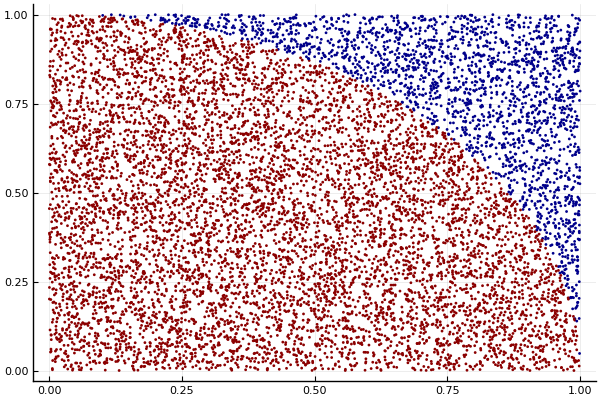
\includegraphics[width=15cm]{images/Ex1.png}
            \caption{Blue dots outisde of circle and red dots inside}
            \label{fig:1}
        \end{figure}

\newpage
	\item Implementation of function for simulating Box-Muller.
        \begin{figure}[H]
            \centering
            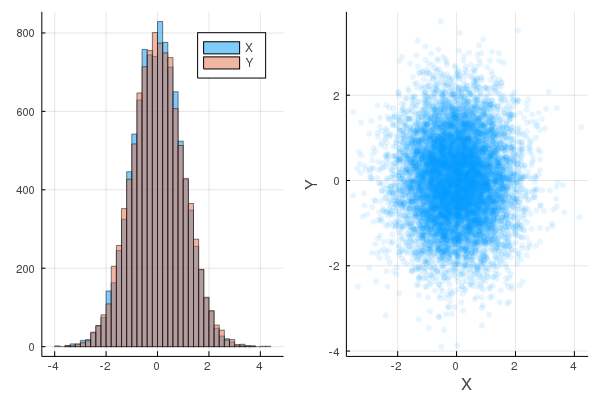
\includegraphics[width=15cm]{images/Ex2.png}
            \caption{In the left the histograms for the distributions
            and in the right a scatter plot to highlight that X and
            Y are independent}
            \label{fig:2}
        \end{figure}
        \lstinputlisting
        {code/Simulation_Exercise2.jl}


	\newpage
    \item Genetic Linkage model, generating histograms.
        \begin{figure}[H]
            \centering
            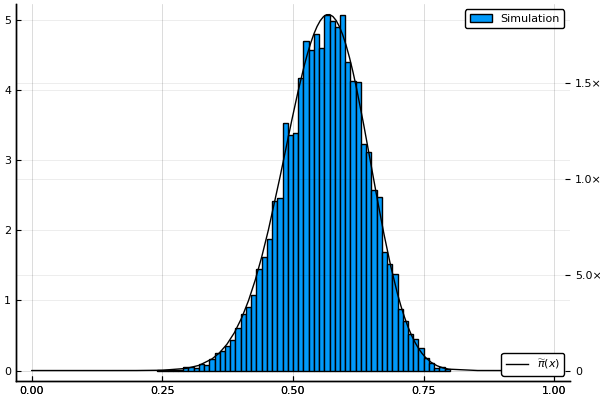
\includegraphics[width=10cm]{images/Ex3_1.png}
            \caption{Histogram for 10.000 samples from
            $p(\theta \mid y_1,...,y_4$ obtained by rejection sampling}
            \label{fig:3}
        \end{figure}

        \begin{figure}[H]
            \centering
            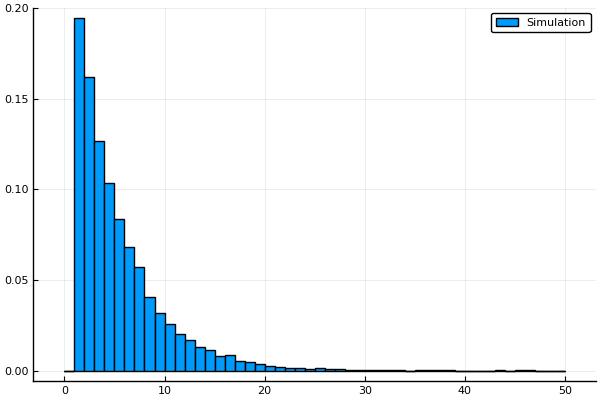
\includegraphics[width=10cm]{images/Ex3_2.png}
            \caption{Histogram of waiting time distribution before
            acceptance}
            \label{fig:4}
        \end{figure}

	\newpage
	\item Implementation of function for Gaussian Mixture.
        \begin{figure}[H]
            \centering
            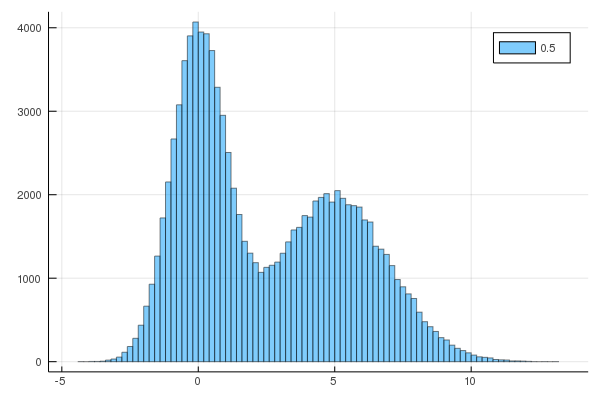
\includegraphics[width=10cm]{images/Ex4.png}
            \caption{Histogram of mixture of Gaussians $N(0,1)$
            and $N(5,2)$, with mixture parameter of 0.5}
            \label{fig:5}
        \end{figure}
        \lstinputlisting
        {code/Simulation_Exercise4.jl}

	\newpage
	\item Let $h(x) = cos(50x)+sin(20x)$
	\begin{itemize}
		\item The exact answer for the integral of $h(x)$ between
		0 and 1 is 0.02435;

		\item Using rejection sampling with an uniform distribution,
		we are able to get an error of roughly 4.31\% for a sample of
		size 1.000.000;

		\item Using an importance sampling with $q ~ Beta(2,2)$ and
		a sample size of 1.000.000, we get an error of roughly 0.62\%.


	\end{itemize}

\end{enumerate}


\newpage
\section*{Appendix (Simulation code)}
\begin{enumerate}[leftmargin=!,labelindent=5pt]
	\item Estimating $\pi$.
        \lstinputlisting
        {code/Simulation_Exercise1.jl}

	\newpage
	\item Box-Muller.
        \lstinputlisting
        {code/Simulation_Exercise2.jl}

	\newpage
	\item Genetic Linkage model.
        \lstinputlisting
        {code/Simulation_Exercise3.jl}

	\newpage
	\item Gaussian Mixture.
        \lstinputlisting
        {code/Simulation_Exercise4.jl}

	\newpage
	\item Rejection and Important Sampling.
        \lstinputlisting
        {code/Simulation_Exercise5.jl}


\end{enumerate}

\end{document}
